\section{Applications}
\label{sec:experiment}


\begin{figure}
	\centering% trim={<left> <lower> <right> <upper>}
%	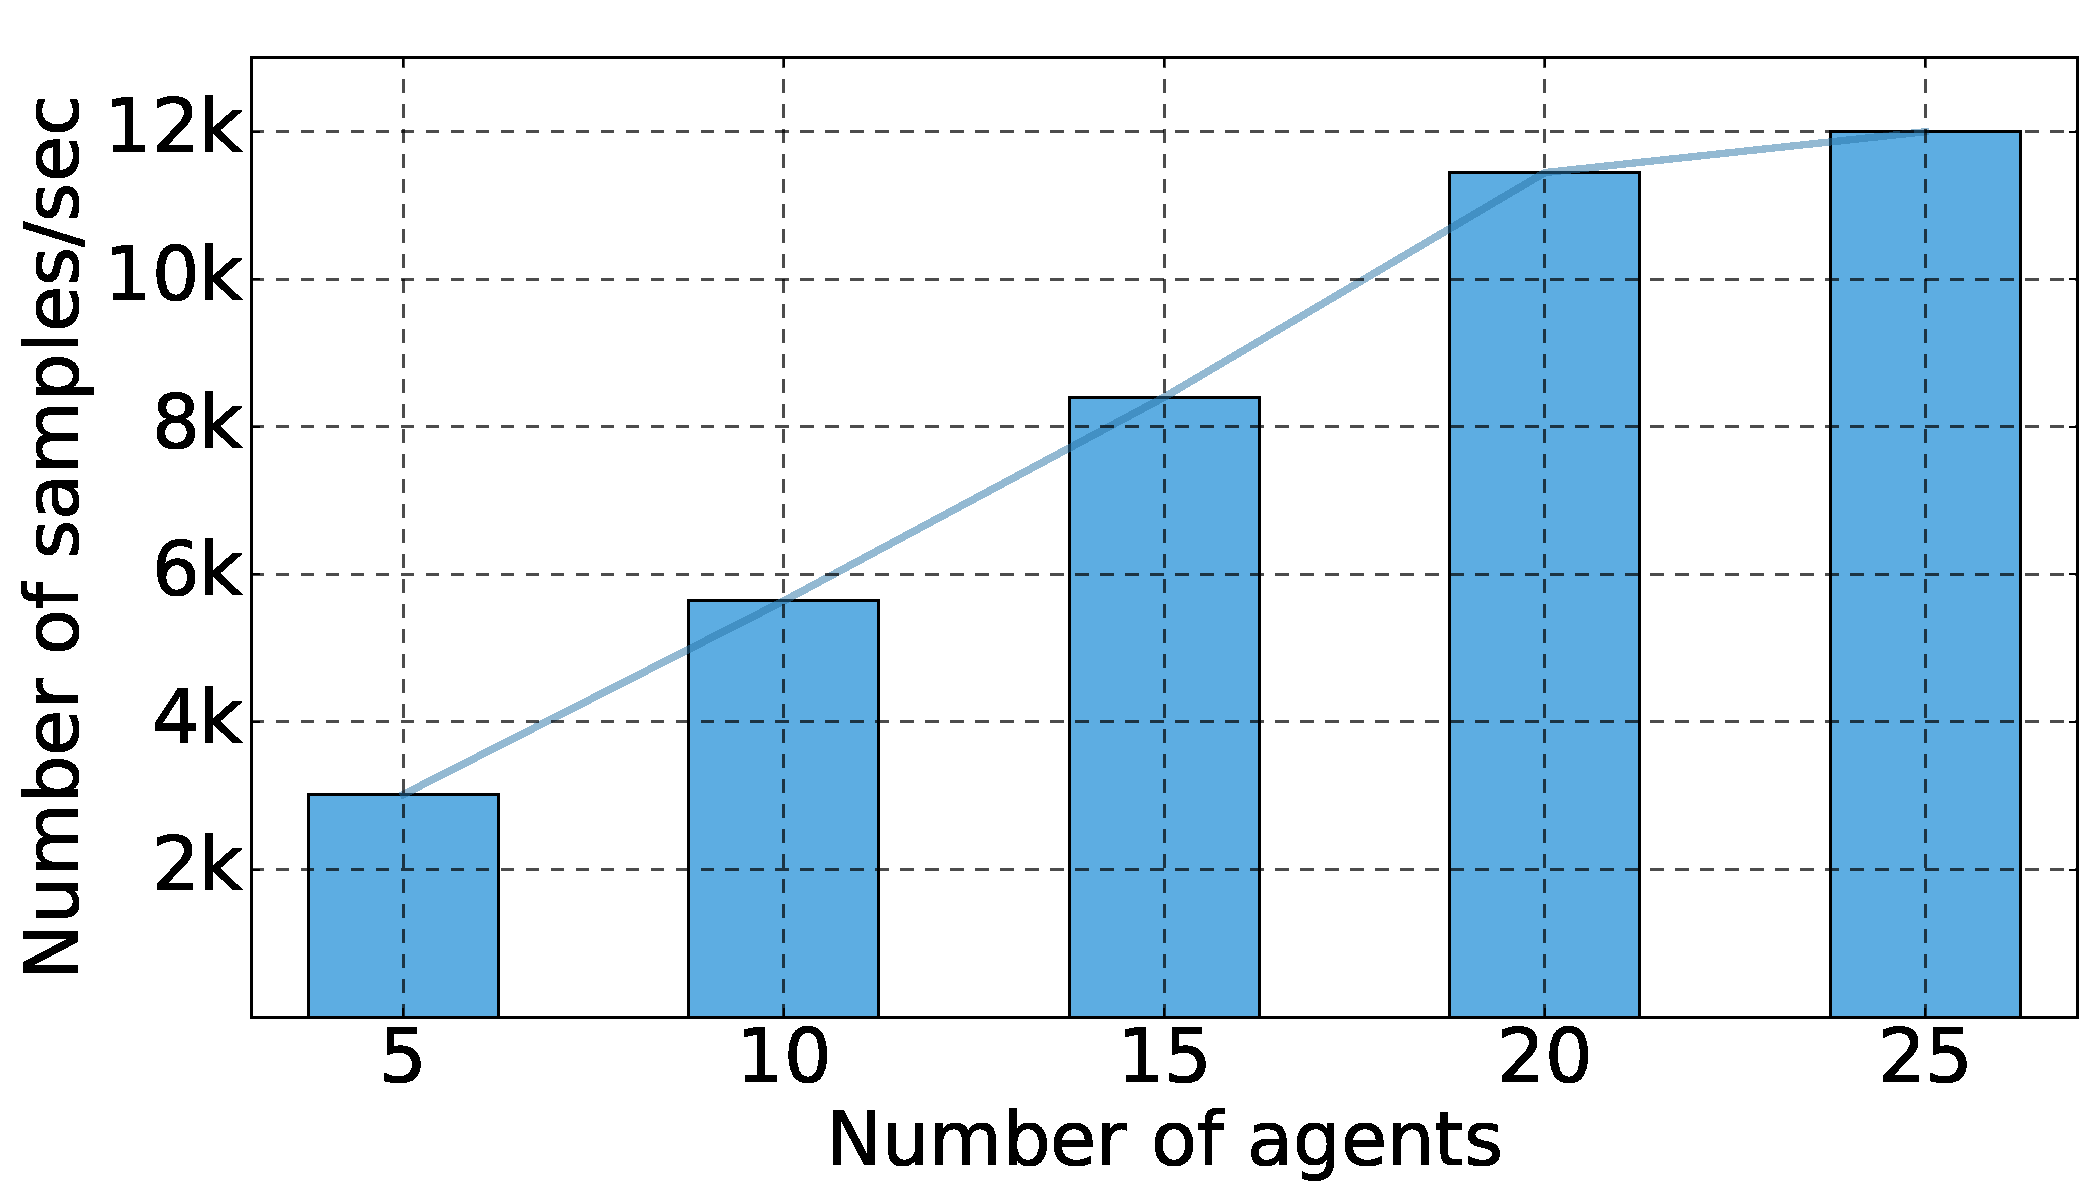
\includegraphics[width=0.42\textwidth]{figures/evaluation/drl_results2}
%		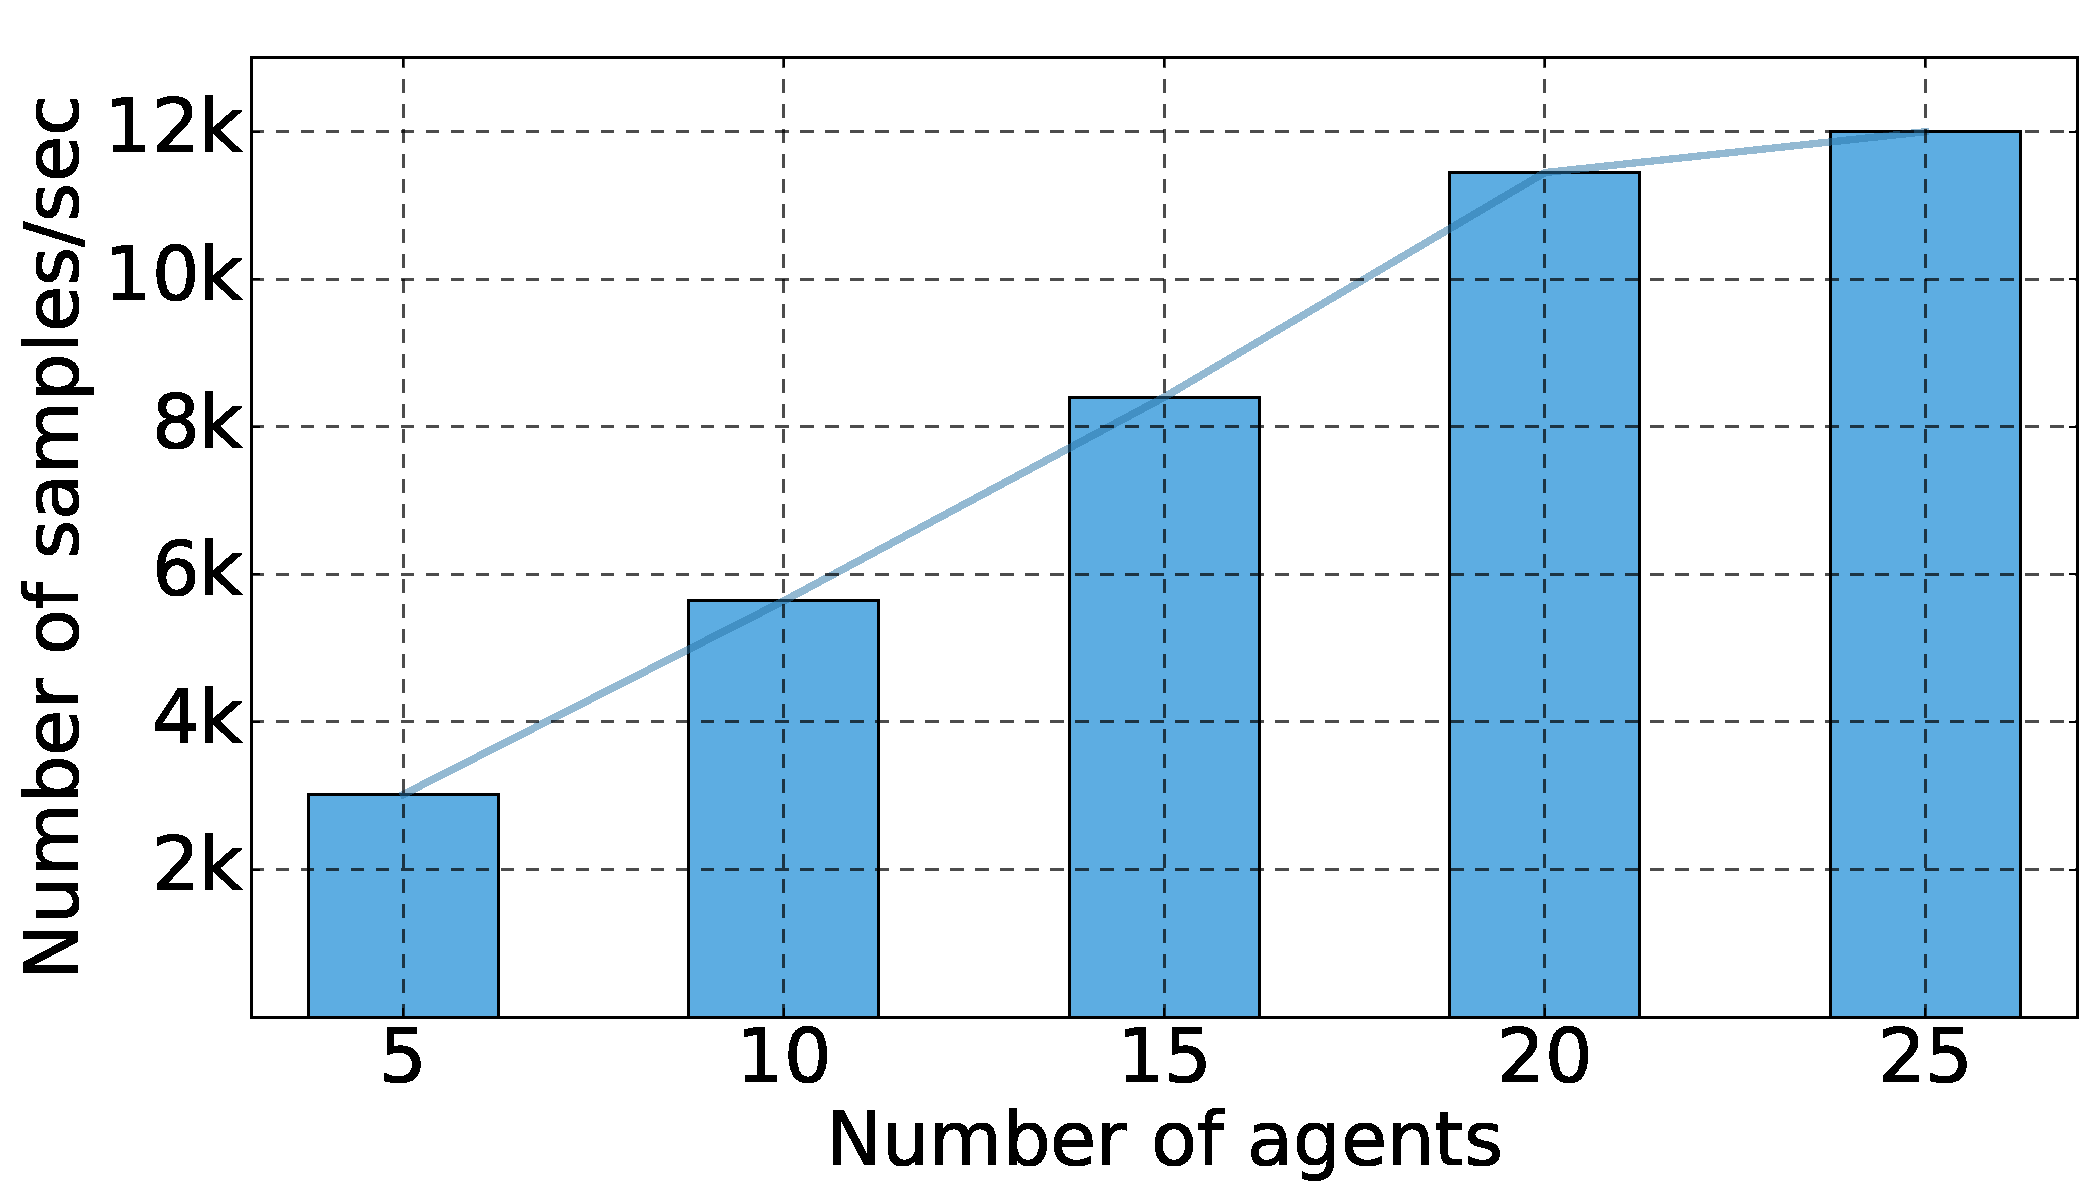
\includegraphics[scale=0.23, trim={0cm 0.39cm 0cm 1.cm},clip]{figures/evaluation/drl_results2}
		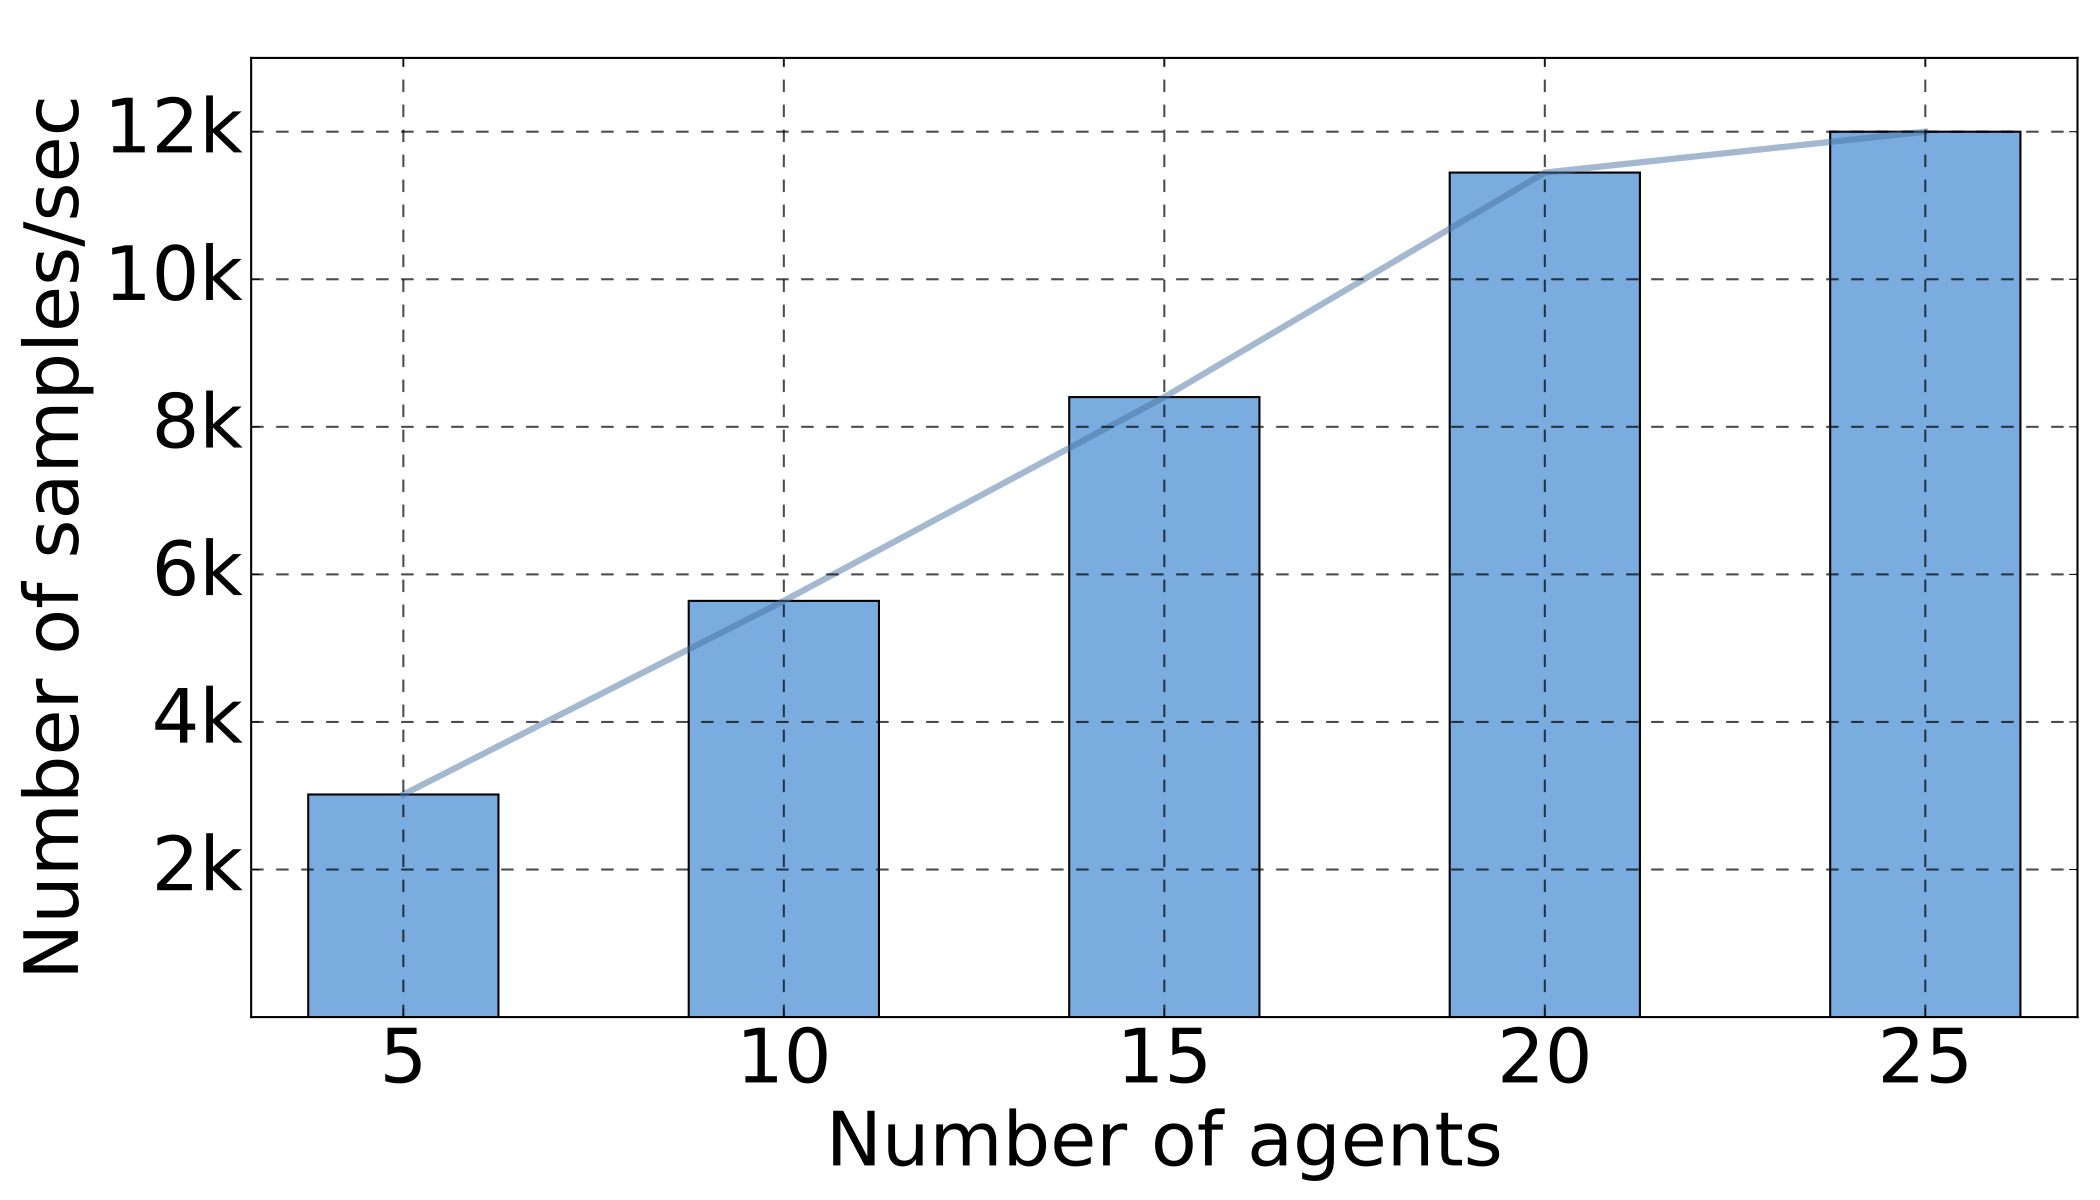
\includegraphics[scale=0.19, trim={0cm 0.39cm 0cm 1.cm},clip]{figures/evaluation/drl_results2.png}
	\caption{Training throughput vs. number of agents used for generating training samples.}
	\label{fig:drl_results}
\end{figure} 

\begin{figure}
	\centering   % trim={<left> <lower> <right> <upper>}
	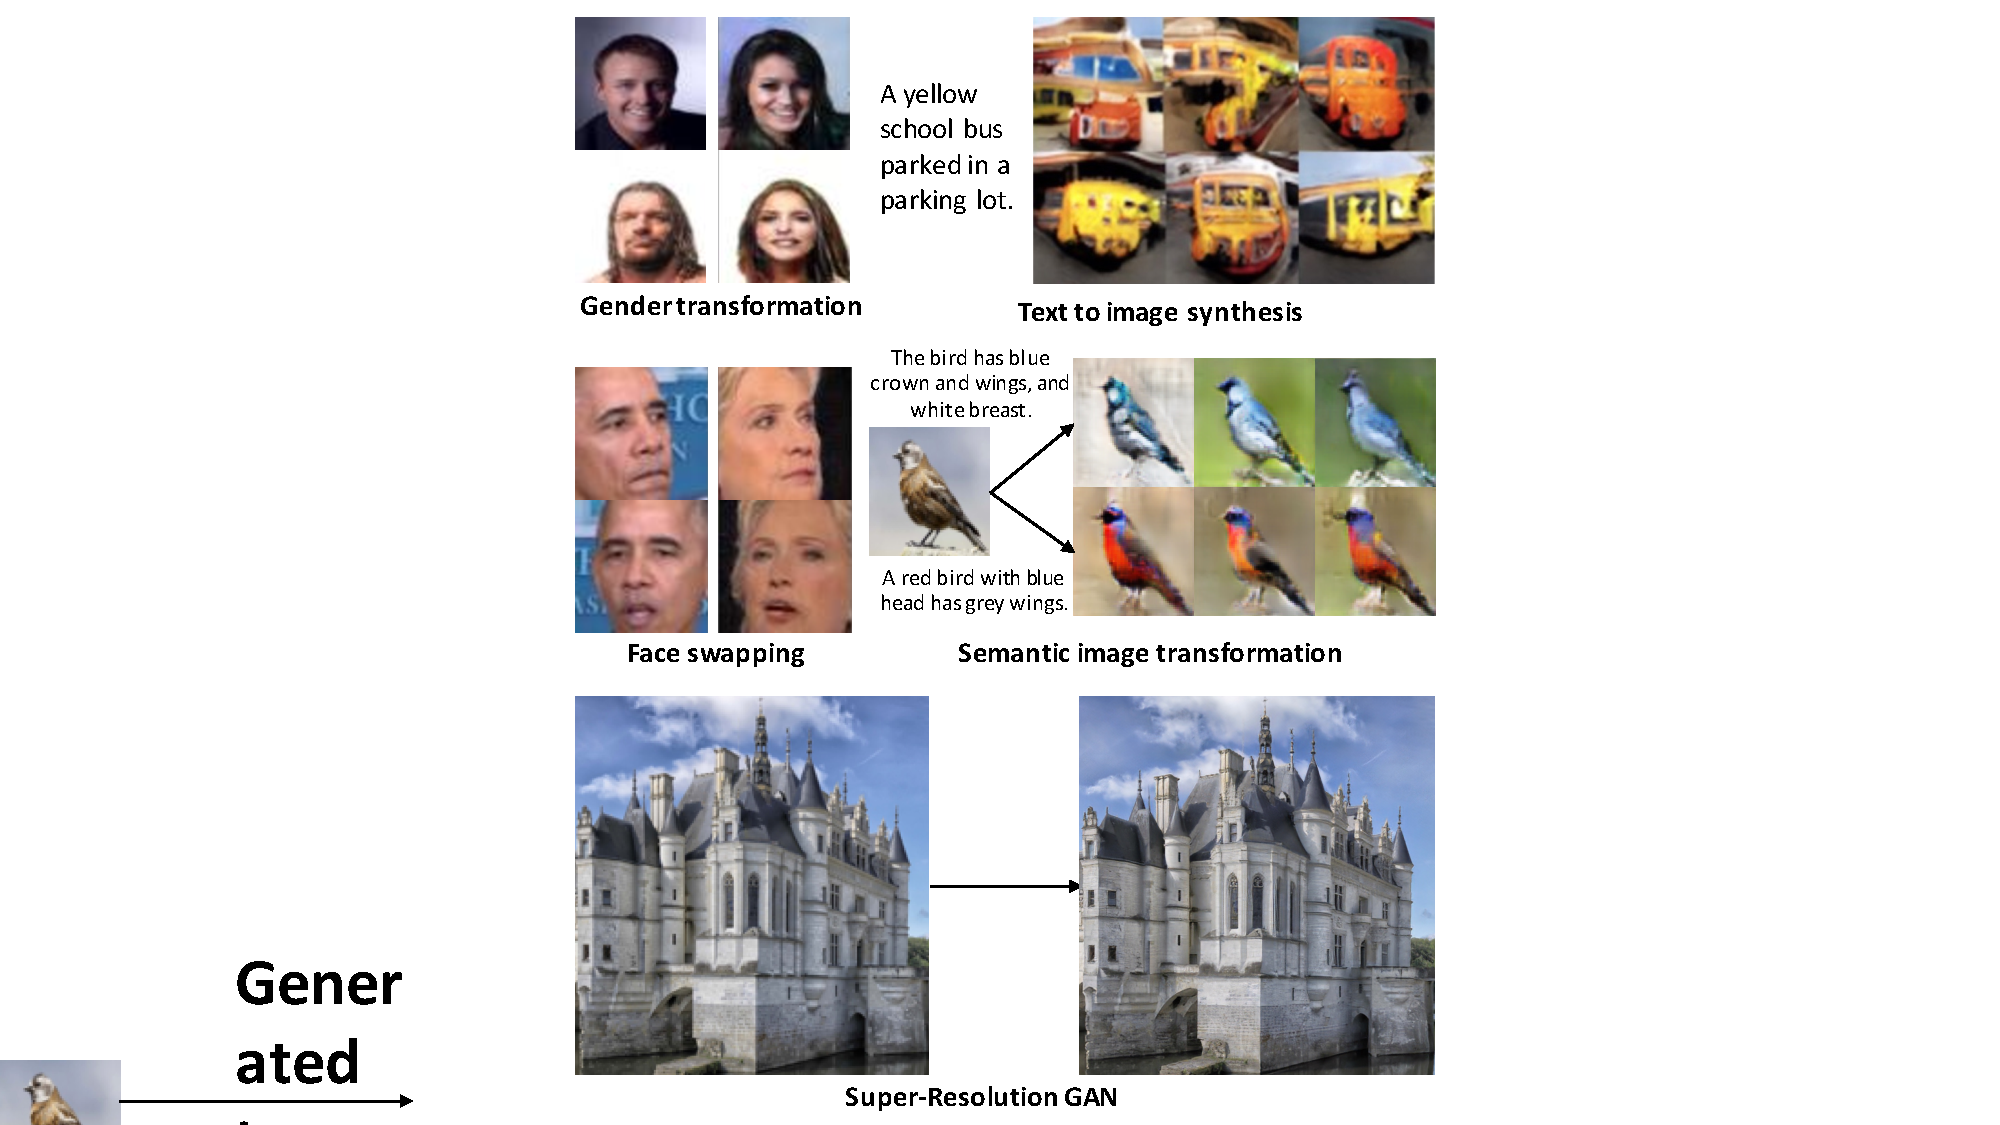
\includegraphics[scale=0.48, trim={9.5cm 0.2cm 9.5cm 0.2cm},clip]{figures/more_app4}
%	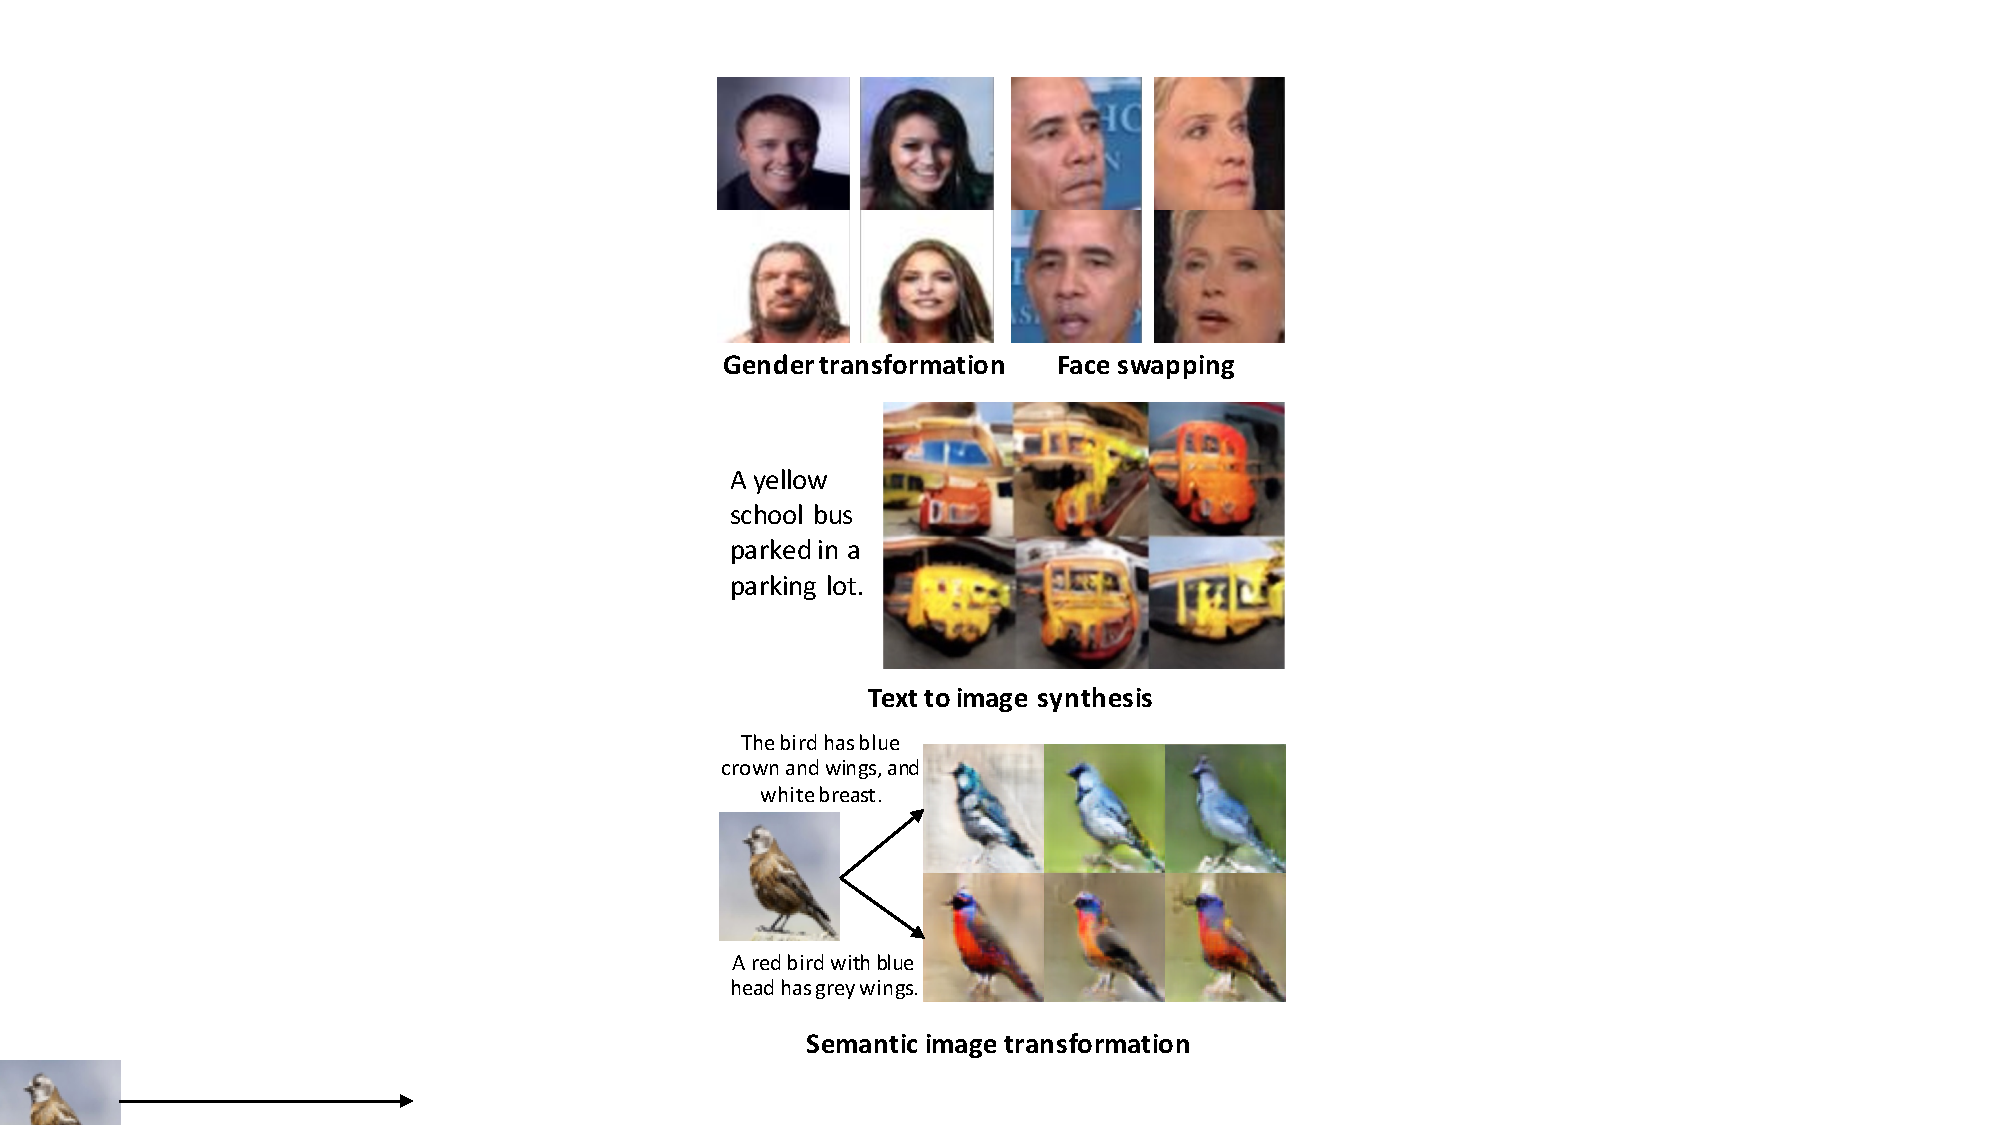
\includegraphics[scale=0.8, trim={12cm 1.0cm 12cm 1.0cm},clip]{figures/more_app3}
	%	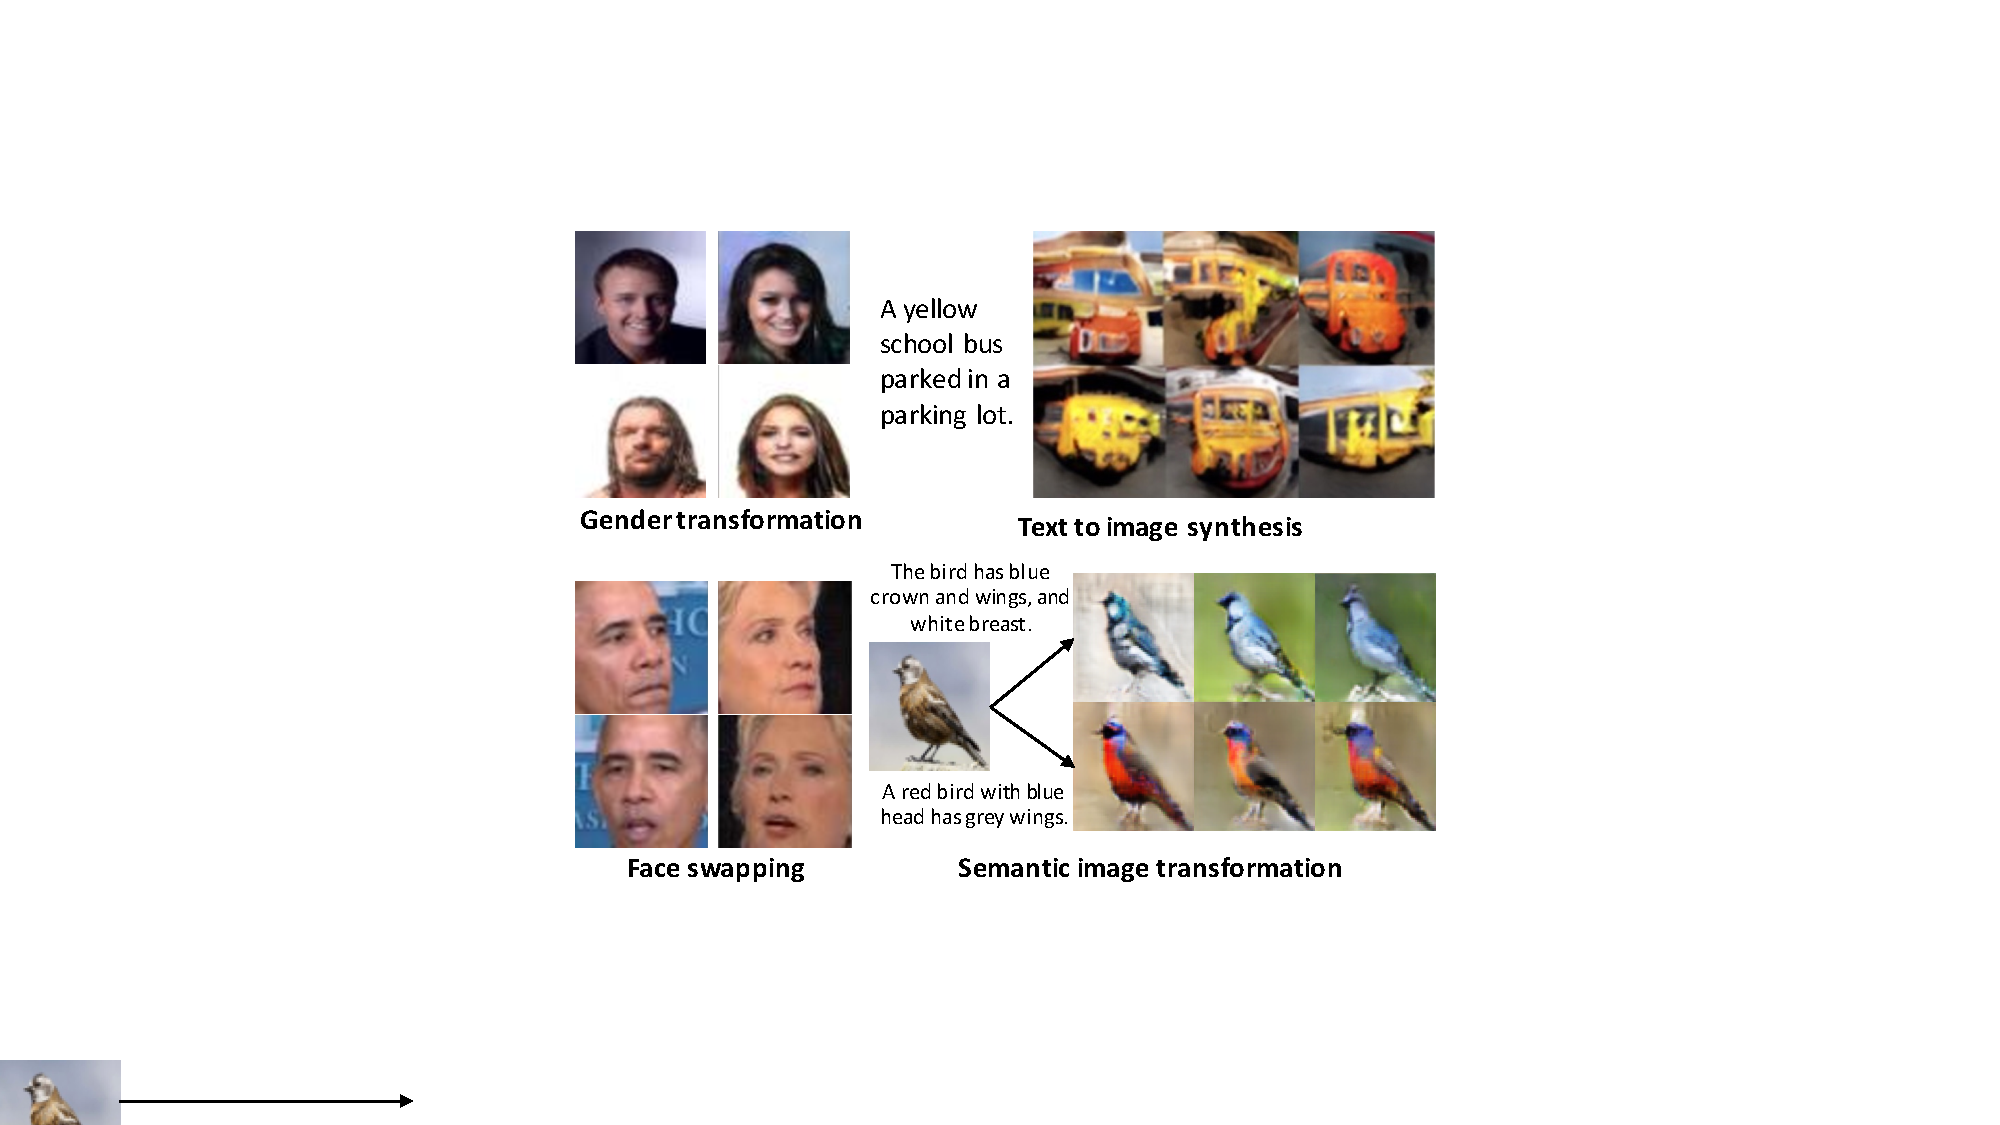
\includegraphics[scale=0.57, trim={9.5cm 4.0cm 9.5cm 4.0cm},clip]{figures/more_app3_2}
	\caption{Highlighted \tl applications.}
	\label{fig:more_app}
\end{figure} 
%\begin{figure*}[h!]
%	\centering   % trim={<left> <lower> <right> <upper>}
%	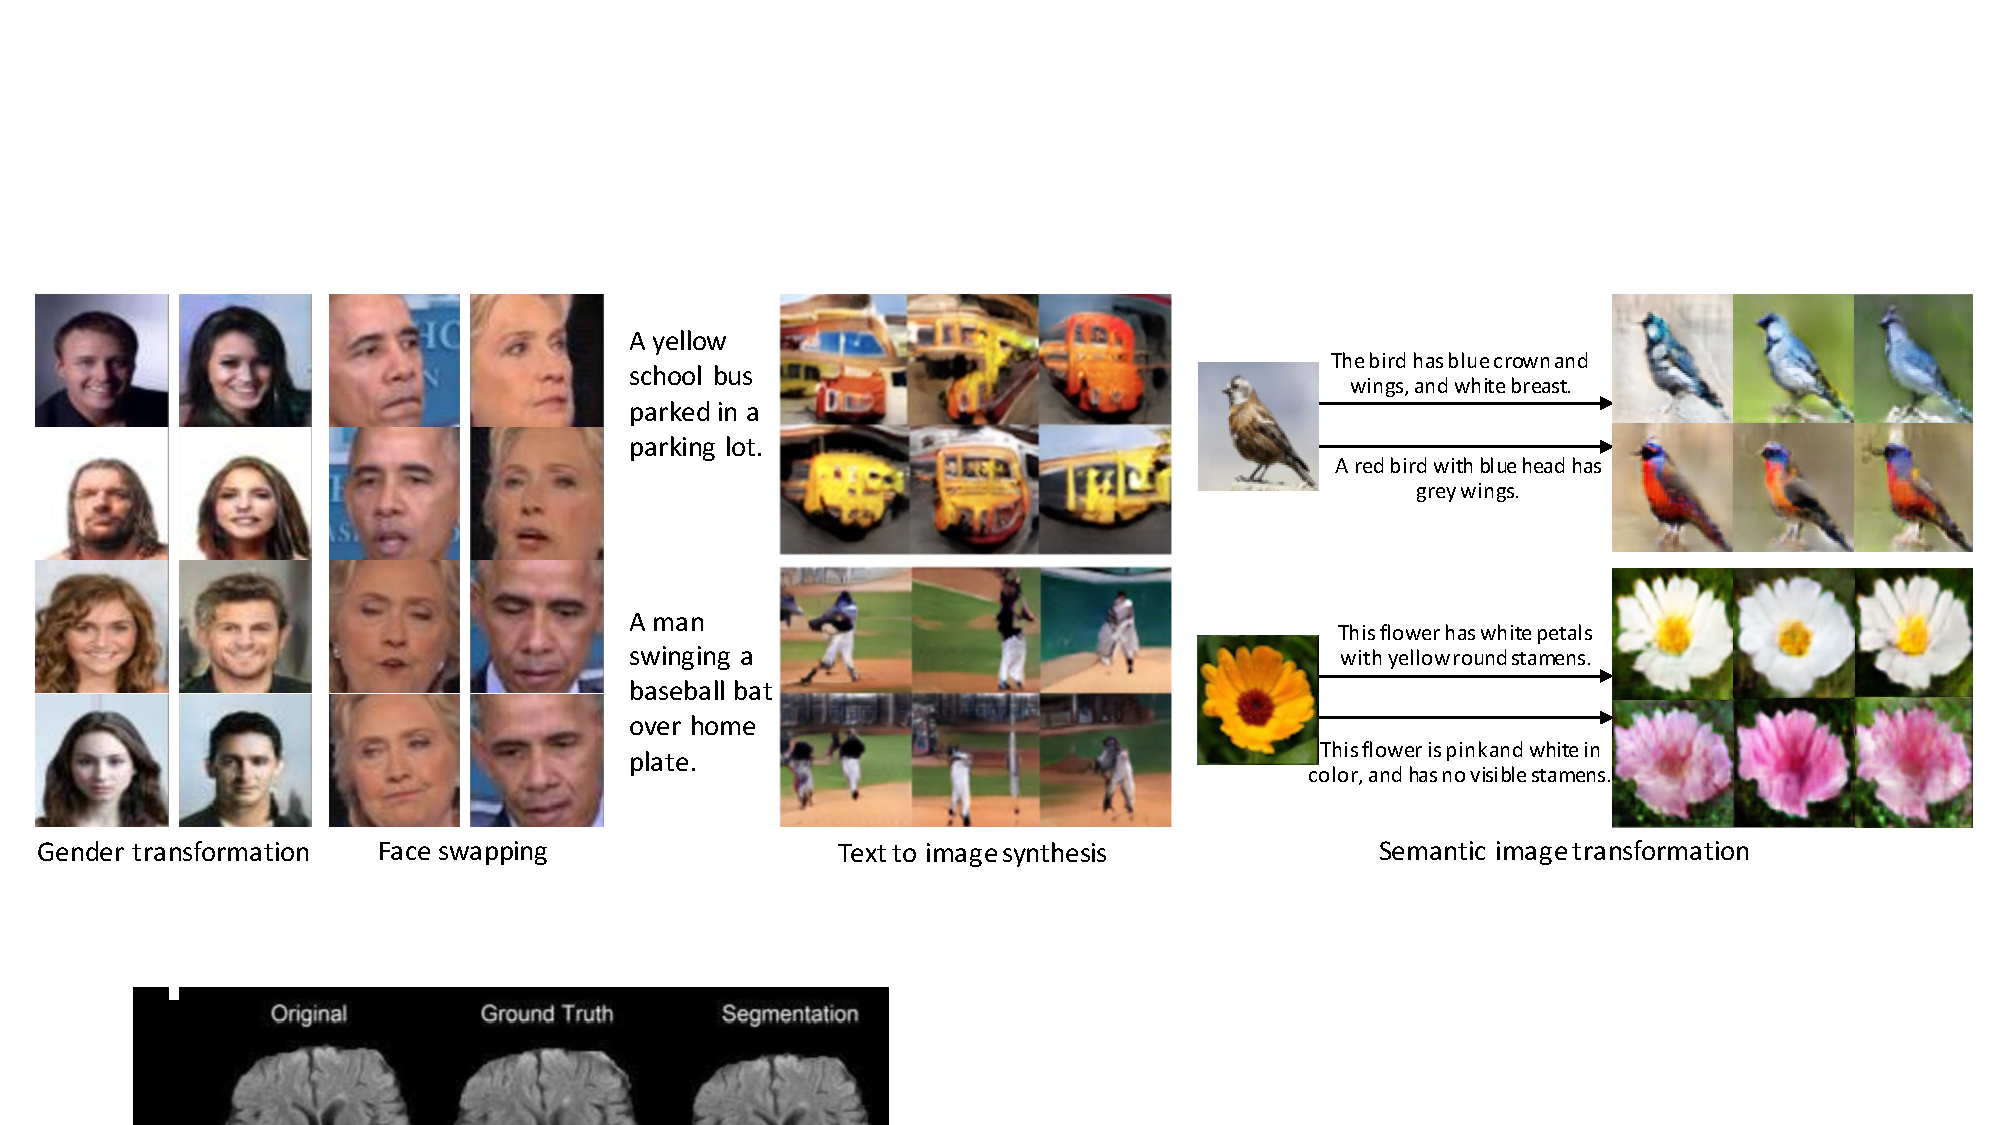
\includegraphics[scale=0.5, trim={0cm 4.0cm 0cm 3.0cm},clip]{figures/more_app}
%	\caption{Highlighted \tl applications.}
%	\label{fig:more_app}
%\end{figure*} 

This section presents a comprehensive study of
deep learning applications that can benefit from using \tl in terms of development efficiency. 
%In this section, we demonstrate some examples that show the advantages of TensorLayer, and some research projects using TensorLayer in Imperial College London. 
Relevant source code is %hosted by a public repository~\footnote{\url{https://github.com/akaraspt/tl\_paper}}.
publicly available on Github~\footnote{\url{https://github.com/akaraspt/tl\_paper}}.

\textbf{Generative adversarial networks.}
%GANs are increasingly popular in multimedia tasks.  %~\cite{radford2015dcgan} 
%A GAN is a dynamic neural network that has two input sources at the discriminator. 
GANs have become a popular deep learning based generative framework for multimedia tasks.
The discriminator network of GANs has two source inputs, which is different from common deep learning architectures. 
\tl enables developers to efficiently construct network architectures of GANs, 
and control the dynamics of a training process, and achieve parameter optimization. 
We take DCGAN~\cite{radford2015dcgan}, an image generation network, 
as an instance to evaluate the helpfulness of \tl. While achieving identical training efficiency, \tl implementation has 187 lines of code (LOC), 
which is 75\% smaller than the published TensorFlow implementation (746 LOC). 
% ours : main.py 96 model.py 67 utils.py 24  / download.py 136
% carpedm20: main.py 76  model.py 406  ops.py 83  utils.py 181 / download.py 147
We use Super-Resolution GAN (SRGAN)~\cite{Ledig2016srgan} as another example. The TensorLayer-based implementation of SRGAN is 526 LOC in length. This is smaller than many other open-sourced implementations that often have more than a thousand LOC.


\textbf{Deep reinforcement learning.} A DRL application is a great example that showcases a joint usage of the layer, model, dataset and workflow modules. 
Specifically, developers can use \tl to build a DRL model, manage model's states between iterations, and create training data that will be constantly generated by concurrent game players.
To demonstrate this, we implement a distributed asynchronous DRL system %~\cite{mnih2016asynchronous}\
 in a cluster that has 10 Gbps connectivity. 
The system trains an agent for playing Atari pong game~\cite{pingpixel2016} on a GTX 980 GPU.
The trainer keeps receiving samples (i.e., observations, actions and rewards)
from game players simulated by \tl agents. 
Trained network models are shared with all players %using the model synchronization function in \tl. 
via the model module of \tl.
Figure~\ref{fig:drl_results} illustrates the scalability of \tl in powering such a system. The training throughput is linearly increasing with more joining agents, until %the GPU finally becomes the bottleneck.
it reaches the maximum capacity of the GPU. 



\textbf{Hyper parameter optimization and cross-validation.}
These two machine learning jobs are necessary for addressing domain-specific problems, 
e.g., medical signal processing~\cite{deepsleepnet2017}, which usually
do not have universally effective models. Hence, they
help developers explore various models and evaluate their performance.
Previously, they were implemented using ad-hoc components. These implementations incurred high maintenance cost, 
and reduced task efficiency due to the cross-component overhead (e.g., serialization and network transfer).
Integrating them with \tl significantly reduces the development and maintenance complexity. 
In addition, experiment results show that \tl can gently increase task parallelism while only incurring
low memory and I/O overhead within the shared data infrastructure. 



\textbf{More applications.}
There are many more applications that have benefited from using \tl. We highlight a few of them here:
multi-model research~\cite{i2t2i2017}, image transformation~\cite{unsupim2im2017, myiccv2017}, and medical signal processing~\cite{braintumor2017, deepsleepnet2017}.
Their results are illustrated in Figure~\ref{fig:more_app}.





